\documentclass[a4paper]{report}
\usepackage{a4wide}
\usepackage[utf8]{inputenc}
\usepackage[T1]{fontenc}
\usepackage{parskip}
\usepackage{hyperref}
\usepackage{epsfig}
\usepackage{background}
\usepackage{mathptmx}

% To avoid tikz error, see https://tex.stackexchange.com/questions/165929/semiverbatim-with-tikz-in-beamer
\makeatletter
\global\let\tikz@ensure@dollar@catcode=\relax
\makeatother

\backgroundsetup{
scale=1,
angle=0,
opacity=1,
contents={
\includegraphics[width=\paperwidth,height=\paperheight]{images/spi-front.jpg}}
}

\hypersetup{
  colorlinks   = true,
  urlcolor     = blue,
  linkcolor    = blue,
  pdfinfo = {
    Title = {SPI Annual Report 2024},
    Author = {Software in the Public Interest, Inc.},
    Keywords = {SPI, free software, open source, FOSS, annual report, charity, non-profit, 501c3},
  }
}

\begin{document}

\title{Software in the Public Interest, Inc.\\
2024 Annual Report}
\date{July XXX, 2025}

\maketitle

\newpage

\backgroundsetup{
scale=1,
angle=0,
opacity=1,
contents={
\includegraphics[width=\paperwidth,height=\paperheight]{images/spi-content.jpg}}
}

\hspace{1em}

To the membership, board and friends of Software in the Public Interest, Inc:

As mandated by Article 8 of the SPI Bylaws, I respectfully submit this annual report on the activities of Software in the Public Interest, Inc. and extend my thanks to all of those who contributed to the mission of SPI in the past year.

  \emph{-- Michael Schultheiss, SPI President}

\newpage

\tableofcontents

\newpage

\chapter{Committee Reports}
\section{Membership Committee}

\subsection{Statistics}

On January 1, 2024 we had 198 contributing and 1422 non-contributing members.  On December 31, 2024 there were 208 contributing members and 1480 non-contributing members.

\chapter{Board Report}
\section{Board Members}

Board members as of January 1, 2024:

\begin{itemize}
\item Michael Schultheiss (President)
\item Stephen Frost (Vice President)
\item Zach van Rijn (Secretary)
\item Héctor Orón Martínez (Treasurer)
\item Joe Conway
\item Forrest Fleming
\item Milan Kupcevic
\item Jonatas L. Nogueira
\item Jeremy Stanley
\end{itemize}

Board members as of December 31, 2024:

\begin{itemize}
\item Michael Schultheiss (President)
\item Jonatas L. Nogueira (Vice President)
\item Zach van Rijn (Secretary)
\item Héctor Orón Martínez (Treasurer)
\item Joe Conway
\item Forrest Fleming
\item Milan Kupcevic
\item Katherine McMillan
\item Jeremy Stanley
\end{itemize}

\section{Board Changes}

Changes that occurred during the year:

\begin{itemize}

\item The terms for Stephen Frost, Milan Kupcevic, and Michael Schultheiss expired in July 2024.  Milan Kupcevic and Michael Schultheiss sought, and obtained, re-election.  We'd like to thank Stephen Frost for his work on the board.  Katherine (Katie) McMillan joined the board as part of the same election.

\item On August 12, 2024 the board voted to appoint the following officers:

\begin{itemize}
\item President: Michael Schultheiss
\item Vice President: Jonatas L. Nogueira
\item Secretary: Zach van Rijn
\item Treasurer: Héctor Orón Martínez
\end{itemize}

\end{itemize}

\section{Elections}

A board membership election was conducted in July 2024.  There were 3 board seats up for election.  Nominations were received from Milan Kupcevic, Katherine (Katie) McMillan, and Michael Schultheiss.  Since there was 3 nominations for 3 board seats, no vote was required and the candidates were elected for a 3 year term.

\chapter{Treasurer's Report}

SPI will publish audited financial statements soon (approximately August 2025).

\chapter{Member Project Reports}

\section{New Associated Projects}

\subsection{Gentoo Linux}

\href{https://www.gentoo.org/}{Gentoo Linux} is a free operating system based on Linux that can be automatically optimized and customized for just about any application or need. Extreme configurability, performance, and a top-notch user and developer community are all hallmarks of the Gentoo experience.

\subsection{Rigs of Rods}

\href{https://www.rigsofrods.org/}{Rigs of Rods} is a free and open source vehicle simulator that uses soft-body physics to simulate the motion destruction and deformation of vehicles.

\subsection{Rocket}

\href{https://rocket.rs/}{Rocket} is a web framework for Rust that makes it simple to write fast, type-safe, secure web applications with incredible usability, productivity and performance.

\subsection{Whisper}

Whisper's mission is to provide free, open-source client and server software that enables participation in spoken conversations by people who have difficulty speaking.

\section{Projects No Longer Associated with SPI}

\begin{itemize}

\item Gallery is no longer active.

\item OpenVAS is no longer associated with SPI.

\end{itemize}

\section{Updates from Associated Projects}

\subsection{Adélie}

\href{https://www.adelielinux.org/}{Adélie} is a lightweight, musl-based, independent Linux platform for desktop and server use, committed to integrity, privacy, and user freedom.

The Adélie Linux distribution continued to deliver on its commitments. In 2024, we released our \href{https://blog.adelielinux.org/2024/12/15/adelie-linux-1-0-beta6-released/}{sixth beta}, which includes new packages, up-to-date toolchains, Rust 1.80, Linux kernel 6.6 LTS, Firefox 128, Xfce 4.20, initial support for Wayland compositors, and initial support to be init-system-agnostic.

Press coverage has been notable. We’ve been featured by \href{https://www.theregister.com/2024/12/20/adelie_linux_1_beta_6/}{The Register} and \href{https://distrowatch.com/weekly.php?issue=20240212}{DistroWatch}, and we’re happy to see retrocomputing enthusiasts and smaller outlets diving in as well.

Over 700 commits by 12 authors went into this release. Bootstrapping remains an active focus for both porting and provenance reasons, details of which can be found in our \href{https://blog.adelielinux.org/2024/12/24/2024-state-of-the-adelie-linux-distribution/}{2024 status report}.
Our self-hosted infrastructure is now fully sustained by generous sponsors and donations, a long time goal and significant milestone.

Thank you to our \href{https://git.adelielinux.org/groups/adelie/-/group_members}{team}, our \href{https://www.adelielinux.org/sponsors/}{sponsors}, and our users for being part of it Follow our \href{https://blog.adelielinux.org/}{blog} and \href{https://www.adelielinux.org/contact/}{social media accounts} to stay informed about our progress.

\subsection{Ankur.org.in}

The activities of the group members have moved ahead in two specific directions of language computing and AI. Over the last six months, the members of the group have been participating as experts for initiatives focused on LLMs for Indian languages. This activity has resulted in prototypes (some under open source license and others not), pilot projects and some degree of reasonable success in demonstrating how well designed AI systems can be effective in classrooms as teaching aids.

The other significant activity we continue to be involved with is digitization of texts and archival. Our engagement here is more as individuals who are available for consultation into a fully formed project.

Over the years \href{https://ankur.org.in/}{Ankur.org.in} has seen the usual trend of contributors moving on to pursue their own specific interests and domains. Sometimes these do not natively align with the focus and mission of language computing that the group was formed around. And as such, we are now at a significantly small set of members who focus on pushing the potential of language computing around more impactful dimensions - especially with AI/ML and LLM related conversations receiving so much focus, attention and discussion.

We are grateful to SPI for being around to provide the organisational infrastructure that makes our work possible and enriches the world.

\subsection{Arch Linux}

\href{https://archlinux.org/}{Arch Linux} is a lightweight and flexible Linux distribution that tries to Keep It Simple. In 2024, the Arch Linux project made significant technological progress and began taking the first concrete steps towards official multi-architecture support.

We welcomed 11 new Arch Linux staff members across various roles, including Package Maintainers, ArchWiki Maintainers, Mirror Admins, Project Maintainers and Support Staff.

An “Arch Linux Ports” RFC has been accepted, establishing the foundation, requirements, and expectations for future secondary architectures. Alongside this, we began work on two critical projects essential for multi-architecture support: a remote signing enclave (signstar) and an automated build service tailored to the needs of our distribution (buildbtw). These initiatives mark the beginning of an exciting future where we aim to further streamline our workflows and expand support for optimized and additional architectures.

Pacman saw two major releases, including version 7.0.0, introducing `autodeps' and enhanced security through the ability to drop privileges when downloading files. Additionally, a new `Landlock' sandbox was implemented to prevent writes outside restricted directories.

Considerable development continued across many of our core projects, with `ArchISO', `arch-boxes', `archinstall', `mkinitcpio', `devtools', and many more receiving multiple updates, new features and enhancements.

The Arch Summit 2024, held on November 23rd and 24th, brought together Arch Linux staff and invited guests for in-depth discussions on critical aspects of our distro. We also maintained strong community engagement with our continued presence at FOSDEM, including a community meetup.

\subsection{Arch Linux 32}

The Arch Linux 32 team continues to make steady progress.

The build system is still building packages, which might even run. Testing resources are currently running low (as are developing hands).

There were no new ISOs this year, mainly due to a broken Python universe.

The i486 sub-architecture is pretty much bit-rotten now.

Most of the binary packages for the i686 and  pentium4 sub-architectures are kept alive with shim packages containing libraries like ICU, boost, etc.

We did some effort to rebuild Python and Python packages as well as keeping Rust working.

\subsection{Battle for Wesnoth}

Battle for Wesnoth is a cross-platform turn based strategy (TBS) game with a high fantasy theme. It features both a variety of single-player campaigns to play as well as online/hotseat multiplayer. Wesnoth's code is licensed under the GNU GPL v2+ and its art and sound assets are licensed depending on when they were added as GNU GPL v2+ (prior to July 30th 2017) or CC BY-SA 4.0 (as of July 30th 2017). Wesnoth has been developed for over two decades by hundreds of contributors.

In 2024 Wesnoth's newest stable series, 1.18, was released. This update included a brand new campaign, an overhaul of an existing campaign to bring it up to modern quality standards, adding a view into the game history data stored in Wesnoth's database so players can search for games and download replays, an achievements system has been added which is also available to content creators, significant improvements were made to the scenario and map editor including new terrains and terrain variations, and a variety of units had their sprite art improved and animations added.

Development continues with the 1.19 series with additional functionality being added to the scenario editor, sprite and portrait art being added or improved, unit and faction balance revisions as well as new units being added, and the start of a major UI modernization effort.

\subsection{Compile Farm}

\href{https://portal.cfarm.net/}{Compile Farm} is a volunteer-run project that maintains a distributed network of diverse computing resources for developers of software with OSI-approved licenses. Machines are owned and hosted by third party sponsors.

In 2024, we are happy to welcome online over 15 new machines, covering {\tt aarch64}, {\tt ppc64le}, {\tt riscv64}, {\tt sparc64}, and {\tt x86\_64} across several different operating systems, and 24 new vetted users.

Please see our \href{https://portal.cfarm.net/news/}{News} page for more information.

\subsection{Debian}

During 2024, the \href{https://www.debian.org/}{Debian} project continued to grow and evolve, thanks to the dedication of its large volunteer community and contributors from around the world.

We made substantial progress toward Debian 13 (``Trixie''), with key foundational changes implemented during the year. Most notably, we completed the transition to 64-bit \texttt{time\_t} on 32-bit architectures, preparing Debian for the Year 2038 and ensuring long-term platform viability. In addition, the long-running effort to merge \texttt{/usr}—unifying system directory layouts—was finalized, simplifying package maintenance and bringing Debian in line with other major distributions.

In line with our release management practices, we published regular point releases for both Debian 11 (``bullseye'') and Debian 12 (``bookworm''). These updates included important security fixes and bug fixes to improve the reliability of our stable distributions.

We welcomed 22 new Debian Developers and 30 new Debian Maintainers in 2024. These new contributors help ensure the sustainability and diversity of our project, and we’re excited to see many of them already actively engaging across teams and packaging efforts.

The Debian community remained vibrant, with a successful \href{https://debconf24.debconf.org/}{DebConf24} held in Busan, South Korea. This was accompanied by several MiniDebConfs around the globe, continuing our effort to reach contributors and users worldwide.

For regular updates and news about what’s going on in the Debian project, visit the \href{https://bits.debian.org/}{Bits from Debian} blog and follow us on the Fediverse and other platforms.

{\em Submitted by Andreas Tille}

\subsection{FFmpeg}

\href{https://www.ffmpeg.org}{FFmpeg} is a complete, cross-platform solution to record, convert and stream audio and video. It is used as the foundation platform of many projects dealing with multimedia, both open source and proprietary, and is used extensively by several web-based multimedia conversion and processing services.

In the year 2024, FFmpeg released version 7.0 `Dijkstra'' in March and the 7.1 point release ``Péter'' in September. A complete list of changes can be found in the \href{https://git.ffmpeg.org/gitweb/ffmpeg.git/blob/HEAD:/Changelog}{changelog}.

FFmpeg joined the \href{https://summerofcode.withgoogle.com/programs/2024/organizations/ffmpeg}{GSoC 2024 program} again enrolling 7 student projects.

In addition, FFmpeg was sponsored for the first time by the \href{https://www.sovereign.tech/tech/ffmpeg}{Sovereign Tech Fund}, an agency financed by the German Federal Ministry for Economic Affairs and Climate Action. A total of 4 projects were undertaken under this sponsorship. There had been developer meetings in February aligned with FOSDEM and aligned with VDD in September.

\subsection{Ganeti}

Already in 2023 Ganeti has been removed from Debian testing, because of the removal of the depended C library libpcre3. While testing sounds not harmful, it has an effect on the derived Ubuntu Distribution. Sadly we failed to fix the problem before Ubuntu 24.04 has been released and in consequence Ganeti is missing there. We were also aware of other breaking changes like broken QEMU disk hotplug even in Debian stable (which nobody seems to noticed) and the Python-3.12 asyncore removal.

On the Haskell side a sponsor stepped in and engaged a Haskell programmer. Besides fixing changed interfaces of used Haskell modules the homegrown make-based build system was migrated to Cabal, also eliminating random/mysterious failures. The reason for Debian removal has been resolved by replacing the used REGEX library at the acceptable cost of loosing PCRE support.

The community fixed many QEMU depredations and breaking changes mostly related to disk handling like command line parameters and QMP hotplug related. And with Python-3.12 asyncore it turns out, that this is available as an external module in Debian Trixie. So technically 2024 Ganeti was back in Debian. Later in 2025 a new release Ganeti-3.1 was created and accepted in Debian.

Personally I'm glad that we managed to go this far since 2017, where Google released Ganeti to the community, however the main task will remain to build a stronger community.

\subsection{Gentoo Linux}

During 2024, Gentoo Linux:

\begin{itemize}

\item \href{https://www.gentoo.org/news/2025/01/05/new-year.html}{Gentoo's 2024 retrospective}

\item Main {\tt ::gentoo} repo: 2.4\% increase in total yearly commits; 19.6\% increase in commits by external contributors.

\item \href{https://www.gentoo.org/news/2024/04/10/SPI-associated-project.html}{joined SPI, and began to wind down the legacy Gentoo Foundation entity.}

\item \href{https://www.gentoo.org/news/2024/02/04/x86-64-v3.html}{Gentoo now also includes x86-64-v3 binary packages, speeding up install and usage on common {\tt amd64} systems}

\item \href{https://www.gentoo.org/news/2024/08/31/KDE-Plasma-6-upgrade.html}{Released KDE Plasma 6 for stable Gentoo}

\item \href{https://www.gentoo.org/news/2024/09/11/Improved-MIPS-and-Alpha-support.html}{Major improvements to MIPS \& Alpha support}

\item \href{https://www.gentoo.org/news/2024/10/07/Arm-Ltd-provides-server.html}{ARM64 \& ARM builds now on a newly donated dedicated ARM64 host, replacing the older Packet.net/Equinix Metal sponsored offering}

\end{itemize}

\subsection{LibreOffice}

In 2024, The Document Foundation (TDF) released two major versions of LibreOffice, starting with LibreOffice 24.2 in February. There were many improvements to the tabbed “NotebookBar” user interface, while styles support was added for comments. Later in the year, LibreOffice 24.8 added many improvements to the Navigator in Writer, including ding cross-references by drag-and-drop items, deleting footnotes and end-notes, and indicating images with broken links. In Calc, the functions FILTER, LET, RANDARRAY, SEQUENCE, SORT, SORTBY, UNIQUE, XLOOKUP and XMATCH were added.

Throughout 2024, TDF and the LibreOffice community organised events and supported free software campaigns around the world. The LibreOffice and Open Source Conference 2024 took place in Luxembourg. There were also two ``Month of LibreOffice'' campaigns, which encouraged LibreOffice users to also become contributors.

\subsection{Manasource}

The united game projects that formed The Mana World Organisation have taken on the name of Manasource to give greater distinction to our original game, The Mana World, which is still actively played and developed. Manasource oversees a large collection of assets and the shared history of the TMW family of projects, seeking to facilitate development of different ideas through its various game titles.

The Mana World has seen one of its founding lead developers return to continue improving the game. An updated version of the original game client (discontinued in 2014 in favour of a fork) will return as TMW's official client soon. Community events and content updates are ongoing.

Source of Mana has finished building its basic Godot infrastructure and is now moving towards game content such as maps, NPCs and more. The game's mission is to refine 20 years of TMW assets into a high-quality finished product with a modern and accessible code base.

Moubootaur Legends continues to release content and innovate with new additions such as the Point of Interest system. A huge variety of content is available and new assets are adapted rapidly to be made available to players.

Find Manasource on our \href{https://forums.themanaworld.org/}{Forums} to stay up to date with news, development and our community!

\subsection{MPI Forum}

During 2024, the MPI Forum work on final preparations for releasing MPI 5.0. This is a major new version of the MPI Standard where the primary improvement is to introduce an Application Binary Interface (ABI), defining a standardized way of providing runtime compatibility between MPI libraries. The new version is expected to be published at our June 2025 meeting. We continue to work on new improvements for future MPI Standard versions and more information can be found at \href{https://mpi-forum.org}{https://mpi-forum.org}.

\subsection{ns-3}

ns-3 is a discrete-event, packet-level network simulator with an emphasis on networking research and education.

In 2024, ns-3 published three software releases of the simulator, thanks to submissions from roughly twenty-five contributors for each release. Many of the model improvements focused on Wi-Fi, LR-WPAN, and cellular technologies, including better support for the latest Wi-Fi standard (Wi-Fi 7), a new Non-Terrestrial Networks channel model and antenna models, and a mobility model supporting geocentric positions and conversion to topocentric coordinate systems. Improvements to the TCP BBR and Cubic models were also made,  ns-3 also mentored three student projects in the 2024 edition of Google Summer of Code. Finally, the annual Workshop on ns-3 (WNS3) was held in June at the Centre Tecnològic de Telecomunicacions de Catalunya (CTTC) in Castelldefels, Barcelona, Spain.  The workshop consisted of ns-3 training sessions, seven technical paper presentations, and a number of invited talks and advanced tutorials.

\subsection{OFTC}

In 2024, OFTC focused on two main initiatives: redesign of its website and the drafting of a new version of its constitution.

\subsection{Open Bioinformatics Foundation}

The \href{https://www.open-bio.org/}{Open Bioinformatics Foundation} (OBF), founded in 2001, is a non-profit, volunteer-run group that promotes open source development and open science in biological research. OBF is led by an \href{https://www.open-bio.org/board/}{elected Board that currently includes 9 members}, with Peter Cock as the president. There have been no changes to the OBF Board in the past year.

In 2024, 10 people were awarded OBF Event Fellowships to attend in-person or virtual events related to open science, including conferences such as Asia \& Pacific Bioinformatics Joint Conference 2024, the 1st Congress by The Spanish Society of Bioinformatics and Computational Biology, the 23rd European Conference on Computational Biology ECCB2024, and Cancer Genomics and Transcriptomics 2024.

We held our 25th annual Bioinformatics Open Source Conference (BOSC 2024) as part of ISMB 2024 in Montréal, Canada, and online. Approximately 200 people participated in BOSC sessions consisting of two keynotes, a panel discussion, 36 talks and 23 posters, covering a wide range of topics in open science and open source bioinformatics. Keynote speakers were Mélanie Courtot on ``The Data Shows We Need Better Data'' and Andrew Su on ``Open Data, Knowledge Graphs, and Large Language Models.'' The BOSC panel discussion, ``Open Source AI/ML: A Game Changer for Bioinformatics?'', included Lawrence Hunter and Thomas Hervé Mboa Nkoudou along with the two keynote speakers as panelists. A \href{https://f1000research.com/articles/13-1100}{full report can be found on F1000}. After BOSC, the 2024 CollaborationFest (CoFest) was held on the campus of Université du Québec à Montréal (UQÀM), including 42 participants who worked together on 10 projects. Outside of the main BOSC conference, OBF and BOSC also sponsored one ISCBacademy talk: Gemma Turon, 2024-03-05, \href{https://www.open-bio.org/2024/03/26/gemma-turon-iscbacademy-talk-video/}{“Ersilia, open source AI/ML for (antimicrobial) drug discovery”}.

The \href{https://www.open-bio.org/}{OBF also re-launched its website} (migrated from WordPress to Hugo), and \href{https://github.com/OBF/newsletter/tree/master/newsletters}{sent out newsletters in March and September 2024}. We always welcome suggestions from the community about relevant content (related to open source / open science) to include in future issues.
\href{https://www.open-bio.org/events/bosc-2025/}{BOSC 2025} will take place July 21-22, 2025 in Liverpool, UK (as part of \href{https://www.iscb.org/ismbeccb2025/home}{ISMB/ECCB 2025}).

\subsection{Open MPI}

The Open MPI community is a collection of academics, researchers, and vendors who continue to develop cutting-edge technology for today’s most-demanding High Performance Computing (HPC) environments.  The community continues to maintain stable release series (v4.1.x and v5.0.x), even while working towards a new release series (v6.0.x).
In 2024:

\begin{itemize}

\item The community released v4.1.7. Further releases are not expected in this series.

\item The community released v5.0.2 through v5.0.6.  More bug-fix releases are expected on this stable release series.

\item A major area of focus is the upcoming v6.0.x series. This series includes several under-the-covers changes to Open MPI’s architecture and infrastructure, as well as several new features from the MPI-4.1 standard.

\end{itemize}

The Hardware Locality ({\tt hwloc}) sub-project released a minor new version (2.11.0) and two additional bug-fix releases, culminating in version 2.11.2.  A new minor release (2.12.0) is expected in 2025.  Continuing prior release norms, the minor releases mainly deal with updates for new hardware and vendor form factors in advanced computing platforms.

\subsection{OpenSAF}

OpenSAF is a high availability middleware, which helps in achieving 99.999\% of service availability to business and mission critical applications. It is the fastest and the most efficient middleware implementation of AIS specifications from SA Forum. OpenSAF is being used mostly in telecom and defence applications worldwide. OpenSAF can detect fault and perform recovery in few milliseconds.

In 2024, we delivered 1 major release: OpenSAF-5.24.02.  More information can be found in the \href{https://sourceforge.net/p/opensaf/wiki/NEWS-5.24.02/}{release notes}.

\subsection{OpenZFS}

OpenZFS is an open-source storage platform that includes the functionality of both traditional file systems and volume manager.

OpenZFS held its annual Developer Summit in October 2024.  This year the conference moved to Portland, OR and we added a 2-day user summit. With 14 presentations and increased attendance from last year, the conference is well into its second decade. Planning for the October 2025 event is underway.

We also published the v2.3.0 release with key features such as RAIDZ Expansion, Fast Dedup, Direct IO, and JSON output, as well as several patch releases with bug fixes and small features.

\subsection{PMIx}

The PMIx organization is a collection of academics, researchers, and vendors who develop and maintain cutting- edge technology for deploying, managing and improving interoperability between most-demanding High Performance Computing (HPC) environmental management software, notably for the deployment and runtime management of distributed applications, and their interoperability with launch managers and batch schedulers. The organization supports the development and release of the PMIx standard, and is closely associated with the Open PMIx and PRTE reference implementations.

In 2024:

\begin{itemize}

\item The organization held 4 Administrative Steering Committee meetings. The meetings included all stakeholders during two 3-hour sessions, during which the eligible ASC members voted on the inclusion and modification of the PMIx standard document. The organization also held elections to renew its chairs and secretaries, and updated bylaw documents.

\item Working groups remained active, proposing amendments to the standard with respect to 1) reviewing use cases and developing illustrative examples; 2) making the document implementation neutral, better separating API definitions and concepts from the reference implementation design; 3) exploring PMIx use in malleable applications and advanced scheduling scenarios that react dynamically to changes at runtime.

\item During the reporting period, the organization published one new revision to the PMIx Standard. PMIx v4.2 is a bugfix release that backports select errata from v5.0 to the backward compatible v4 line of the standard. Work also began on the next release, which aims to promote several provisional items to full stable status.

\end{itemize}

\subsection{POCO}

In 2024, POCO Team released several minor and one major release (1.14.0) in December: \href{https://github.com/pocoproject/poco/releases/tag/poco-1.14.0-release}{See on GitHub}.

The 2024 releases included security fixes, major improvements to the Data::ODBC library and upgrades to the most recent versions of the embedded libraries.

{\em Submitted by Aleksandar Fabijanic}

\subsection{PostgreSQL}

PostgreSQL is a popular free software relational database system, built on the principles of extensibility, security, and robustness. Our community thrives around a wide ecosystem of open source projects that complement the core server, including administrative tools, backup solutions, driver software such as JDBC, and community-operated infrastructure.

Our flagship release in 2024 was PostgreSQL 17, which introduced powerful new features aimed at improving performance, security, and usability. It includes major vacuum memory improvements, making maintenance of large (TB+) tables significantly more efficient. Logical replication is now easier to manage, supporting smoother upgrades and improved high availability. New SQL/JSON functions like JSON\_TABLE enhance JSON handling, while backup and monitoring tools now offer more detailed insights and flexibility. Security has also been upgraded, with new TLS handshake options and a predefined maintenance role.

We continue to see strong growth in our user base, with PostgreSQL once again receiving top marks in the 2024 edition of Stack Overflow’s Developer Survey. We also made good use of our SPI funding—supporting our participation in Google Summer of Code, investing in project infrastructure, and helping revamp our annual developers’ conference.

\subsection{Privoxy}

In 2024, wolfSSL support was committed to git and tests were added that leverage the curl test suite. The work was funded using donations collected by SPI.

\subsection{Rigs of Rods}

In 2024, the march for progress continued. We saw significant improvements to game stability and performance along with plenty of new features to make the modding experience more engaging and easier to use for new players. A major highlight is the new vehicle tuning system, featuring a graphical interface and the {\tt .addonpart} format for easier customization. Dashboards also received a major overhaul, with smoother input, a new .dashboard mod type, and fixes to long-standing HUD issues. The revamped T-menu now unifies various vehicle tools into a single panel, streamlining user interaction. Terrain editing was improved with direct {\tt .tobj} file support, and new mod types like {\tt .assetpack} and gadget simplify content distribution. And finally, we joined SPI in 2024!

\subsection{Swathanthra Malayalam Computing}

In 2024, Swathanthra Malayalam Computing (SMC) maintained its strong involvement in Malayalam computing initiatives. The majority of our technical project activities centered on maintenance and user support. We released updated versions of our fonts and various software projects, including the release of Indic Keyboard v3.6. Our Telegram channel experienced significant engagement and welcomed new users of our tools. We continued our practice of publishing monthly reports to keep the public informed about our activities.

Our community members actively participated in diverse events organized by organizations such as OpenStreetMap, Wikimedia Foundation, Drupal, Debian, and the Indic Digital Archive Foundation. Specifically, our members contributed to State of the Map Kerala, Debutsav 2024, DebConf 2024, Wikimania 2024, IndiaFOSS 2024, WordCamp Kerala 2024, and the Wikimedia Technology Summit 2024. A newly redesigned SMC website was launched in September. We contributed to academic discourse by publishing and presenting papers at conferences including Grapholinguistics 2024 and Empirical Methods in Natural Language Processing 2024. SMC's Annual General Body Meeting took place on September 29, 2024, at the PG Centre in Thrissur. During this meeting, a new executive committee was elected. Additionally, we successfully submitted our long-pending compliance documents as per government regulations for non-profit Science and Technology societies.

\subsection{systemd}

Systemd is a suite of basic building blocks for a Linux system. It provides a system and service manager that runs as PID 1 and starts the rest of the system. In 2024 we published two major releases of systemd and 66 point releases with bug fixes. We merged 7352 commits (up from 6814 in 2023) from a total of 419 contributors. We organized a micro-conference at \href{https://lpc.events/event/18/sessions/206/#20240919}{Linux Plumbers in September}, we organized the \href{https://uapi-group.org/docs/minutes/2024-09-24__image-based-linux-summit/}{Image-Based Linux Summit} and we participated in \href{https://cfp.all-systems-go.io/all-systems-go-2024/schedule/}{All Systems Go!} in Berlin in September. We continue to hold a biweekly maintainers meeting and the project is maintaining a steady pace of development.

\subsection{Translatewiki.net}

\href{https://translatewiki.net/}{Translatewiki.net} is an online translation platform for free and open-source projects, powered by a global community of volunteer translators. In 2024, we approved 1 130 new translators and added support for 42 new languages, bringing our total to 667 locales.

On the development side, we rolled out several major improvements:

\begin{itemize}

\item Notifications: Translators can subscribe to alerts for new things to translate in projects they follow.
\item Automated exports: Our translation export pipeline is now fully automated, and regular \href{https://translatewiki.net/wiki/Dumps}{dumps} of all \href{https://translatewiki.net/}{translatewiki.net} translations are available for download.
\item Platform upgrade: We’ve migrated our infrastructure from Debian 11/PHP 7 to Debian 12/PHP 8 for better performance and security.

\end{itemize}

\subsection{Whisper}

The Whisper Project’s goal is to put high-quality assistive technology, at no cost, into the hands of people who find it difficult or impossible to speak, so that they can participate fully in individual and group conversations with those who can.

In 2024, our work was focused on \href{https://apps.apple.com/us/app/whisper-talk-without-voice/id6446479064}{Whisper - talk without voice}, an iOS/macOS app targeted primarily at the ALS and other communities where someone’s typing as well as their voice is restricted. Whisper works by presenting a “Whisperer’s” keystrokes, in real time, on the screens of one or more “Listener” devices (called “buddy screens” in the ALS community). We released several versions of Whisper on the Apple App Store, introducing many features requested by the user community, including:

\begin{itemize}

\item Bluetooth connectivity, allowing nearby listeners to connect their devices to the conversation automatically.
\item Text-to-speech generation, allowing people without devices to know what the Whisperer is typing.
\item Named conversations, each with a URL, allowing Whisperers to control who is allowed into their conversation.
\item Internet connectivity, allowing remote Listeners with an audio or video connection to participate in conversations.
\item Web-based listening, so that Listeners can listen in their browser on any device.

\end{itemize}

In 2025, we are focused on expanding support to the head-and-neck cancer community, and are cooperating with Washington University in St. Lous on a research study focused on total laryngectomy patients. To that end, we are working on a new app \href{https://apps.apple.com/us/app/in-my-voice/id6742593911}{In My Voice} that provides text-to-speech in an AI-generated “cloned” voice of the patient using a variety of text-to-speech technologies, both open-source and commercial. This app, and its data-collecting back-end server, will be used in the study to measure whether patients prefer using this technology relative to the “electro-larynx” technology already available. The goal is to convince insurance companies that quality-of-life is improved by offering these patients text-to-speech capabilities, so that the companies will fund the necessary infrastructure.


\appendix
\chapter{About SPI}

SPI is a non-profit organization which was founded to help organizations develop and distribute open hardware and software. We encourage programmers to use the GNU General Public License or other licenses that allow free redistribution and use of software, and hardware developers to distribute documentation that will allow device drivers to be written for their product.

SPI was incorporated as a non-profit organization on June 16, 1997 in the state of New York. Since then, it has become an umbrella organization for projects from the community.

In 1999, the Internal Revenue Service (IRS) of the United States government determined that under section 501(a) of the Internal Revenue Code SPI qualifies for 501(c)(3) (non-profit organization) status under section 509(a)(1) and 170(b)(1)(A)(vi). This means that donations made to SPI and its supported projects are tax-deductible as charitable donations for US taxpayers.

\newpage

\pagestyle{empty}

\backgroundsetup{
scale=1,
angle=0,
opacity=1,
contents={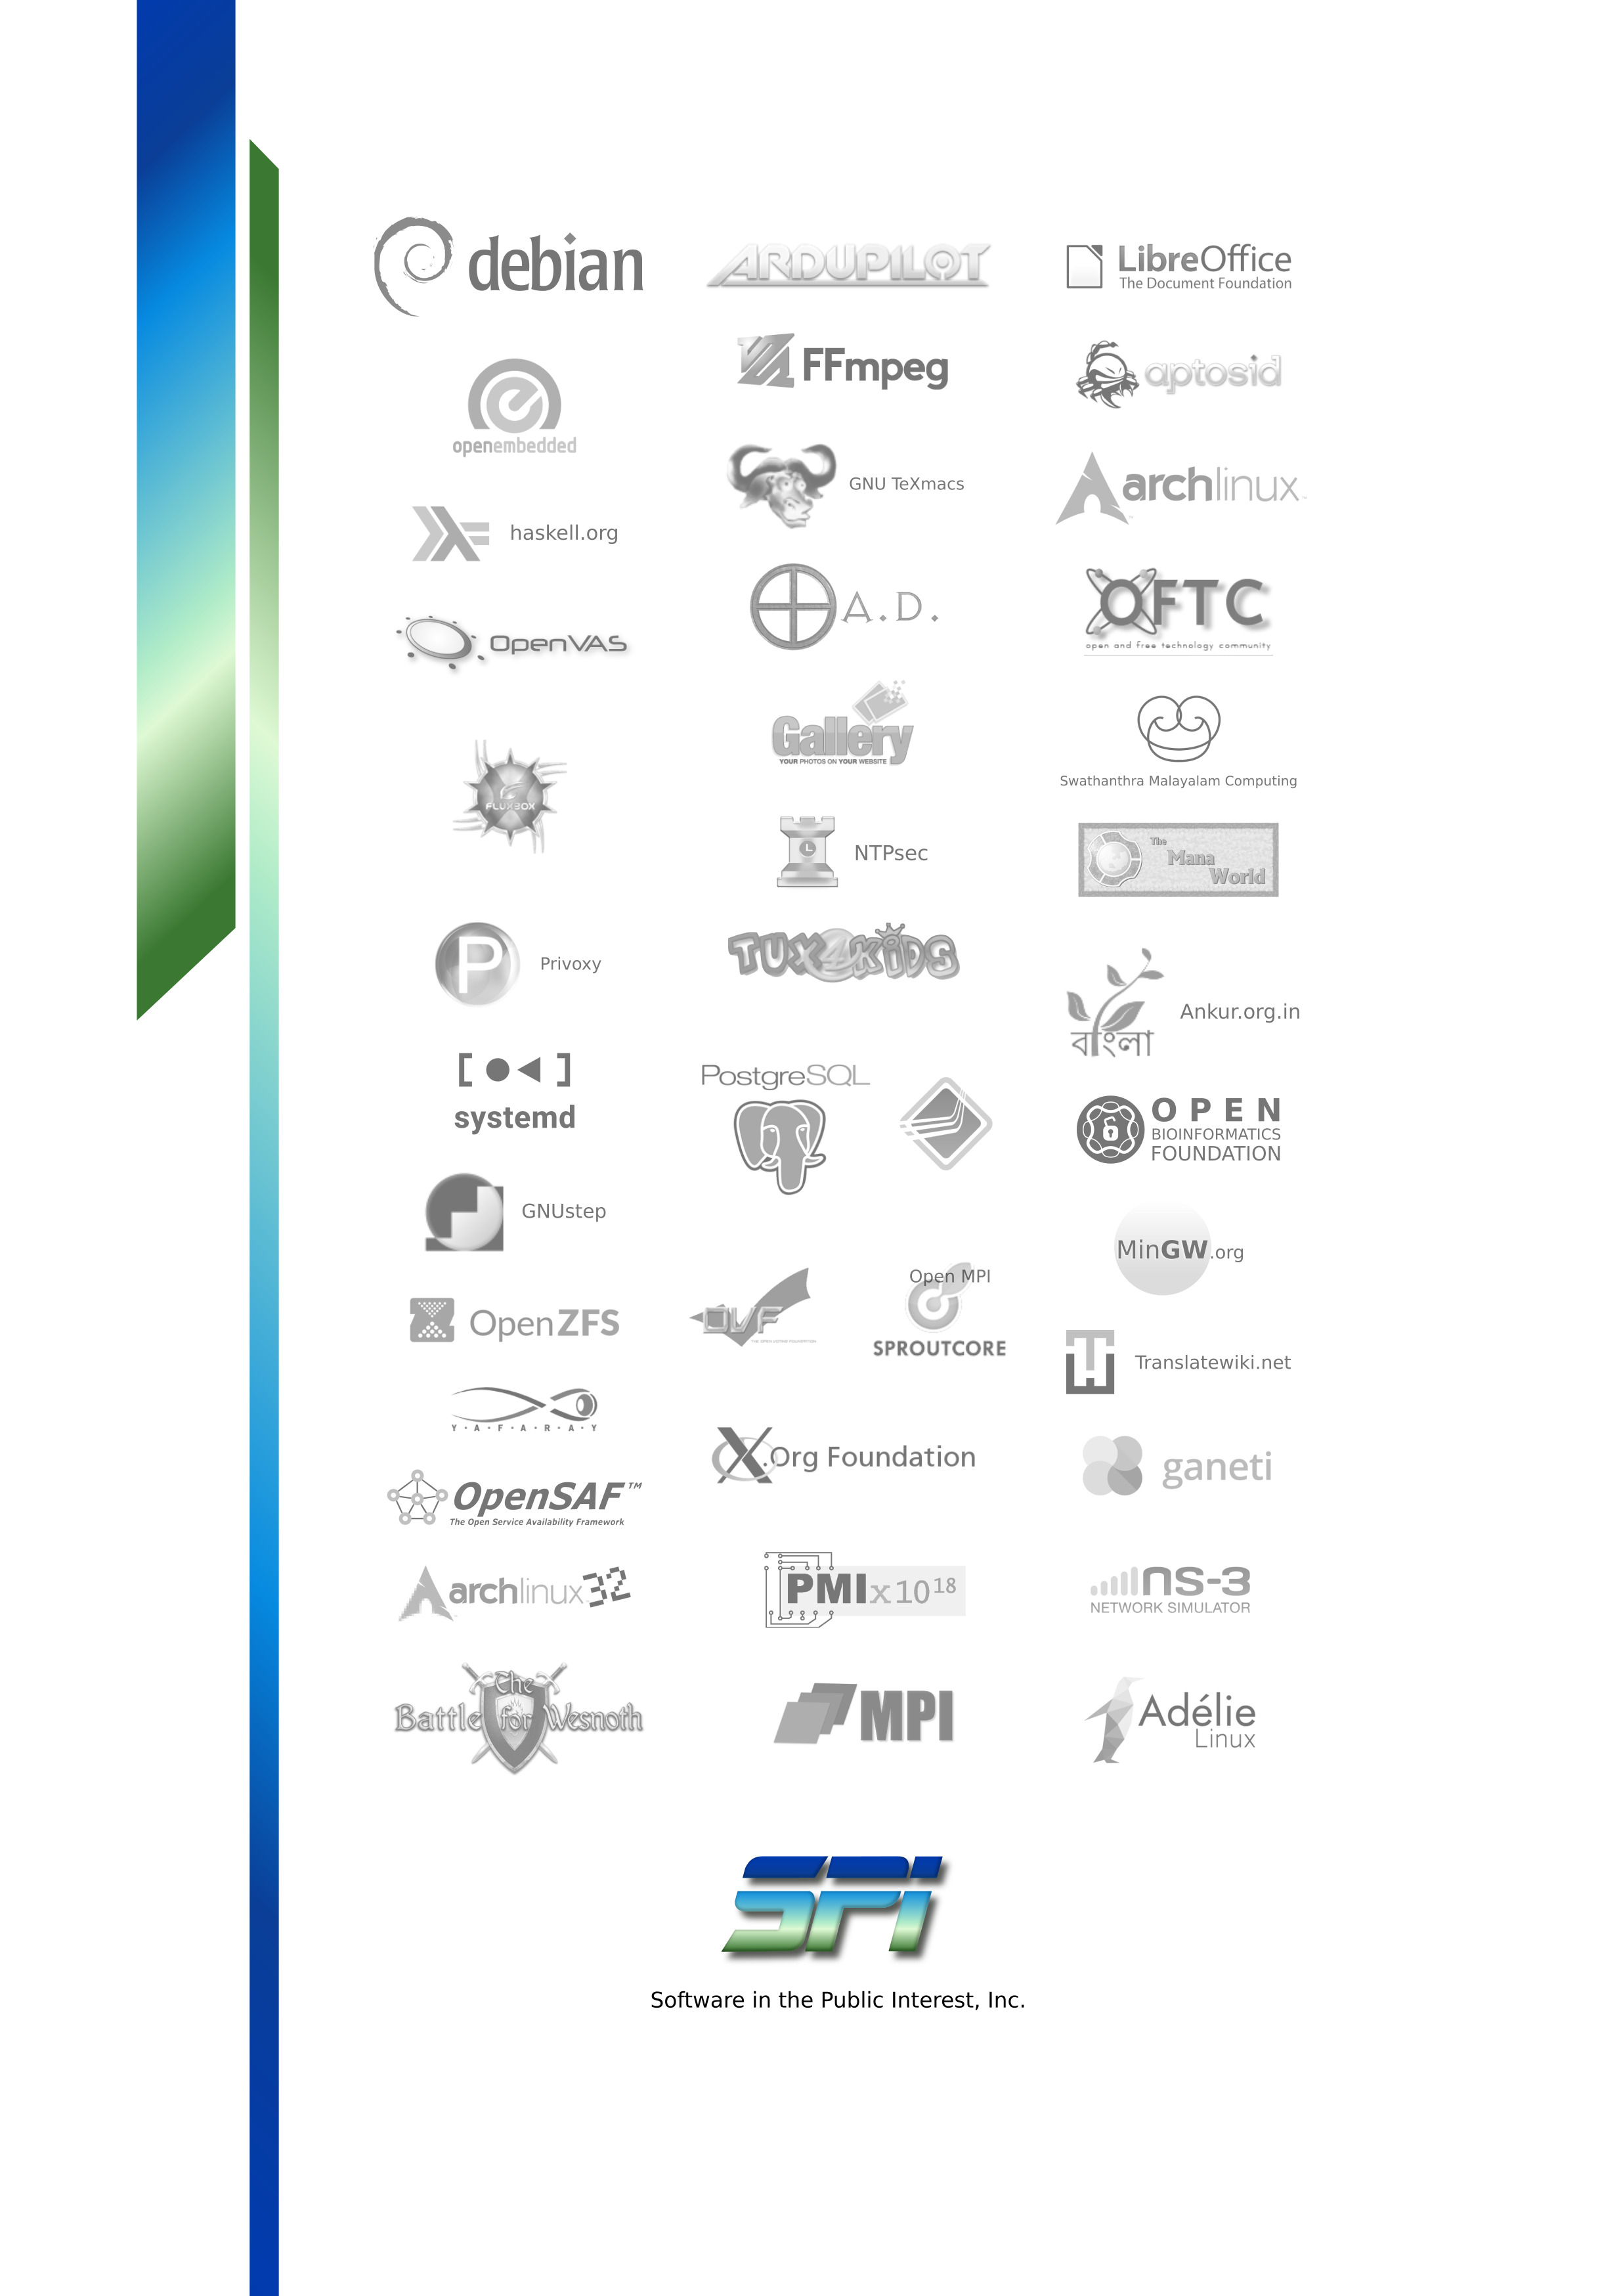
\includegraphics[width=\paperwidth,height=\paperheight]{images/spi-back-2022.jpg}}
}

\null

\end{document}
% Keep this at the bottom, thanks.
% Local Variables:
% TeX-master: "report"
% End:
